\subsection{Transportation Burden}

\begin{frame}
	\frametitle{Haversine Formula}
	Calculates the 'great-circle' distance between two coordinate points\\
	* Coordinate data from Wikidata
	\begin{align} 
	\Phi_1,\Phi_2&= \mbox{latitude in radians}\\
	\lambda_1,\lambda_2 &= \mbox{longitude in radians}\\
	\Delta\lambda &= \left|\lambda_1 - \lambda_2\right|\\
	\Delta\Phi &= \left|\Phi_1 - \Phi_2\right|\\
	a&=\sin^2(\Delta\Phi)+\cos(\Phi_1)\cos(\Phi_2)\sin^2{\left(\frac{\Delta\lambda}{2}\right)}\\
	c &= 2 \cdot arctan2(\sqrt{a},\sqrt{1-a})\\
	d &=  (6,371km) \cdot c
	\end{align}
	
\end{frame}

\begin{frame}
	\frametitle{MTHM*km Calculation}
	\begin{align}
	b_i &= m_id\\
	B &= \sum_i^N b_i\\
	\intertext{where}
	b_i &= \mbox{spent fuel transport burden from facility i [km]]}\\
	m_i &= \mbox{mass of spent fuel at facility i [MTHM]}\\
	B &= \mbox{total spent fuel transport burden [MTHM*km]}\\
	N &= \mbox{total number of facilities with spent fuel on site.}
	\end{align}
\end{frame}

\begin{frame}
	\frametitle{Transportation Burden}
	MTHM of waste in each reactor (data from EIA 2011 Survey - GC859 \cite{domenico_gc-859_2016})
	\begin{figure}[htbp!]
		\begin{center}
			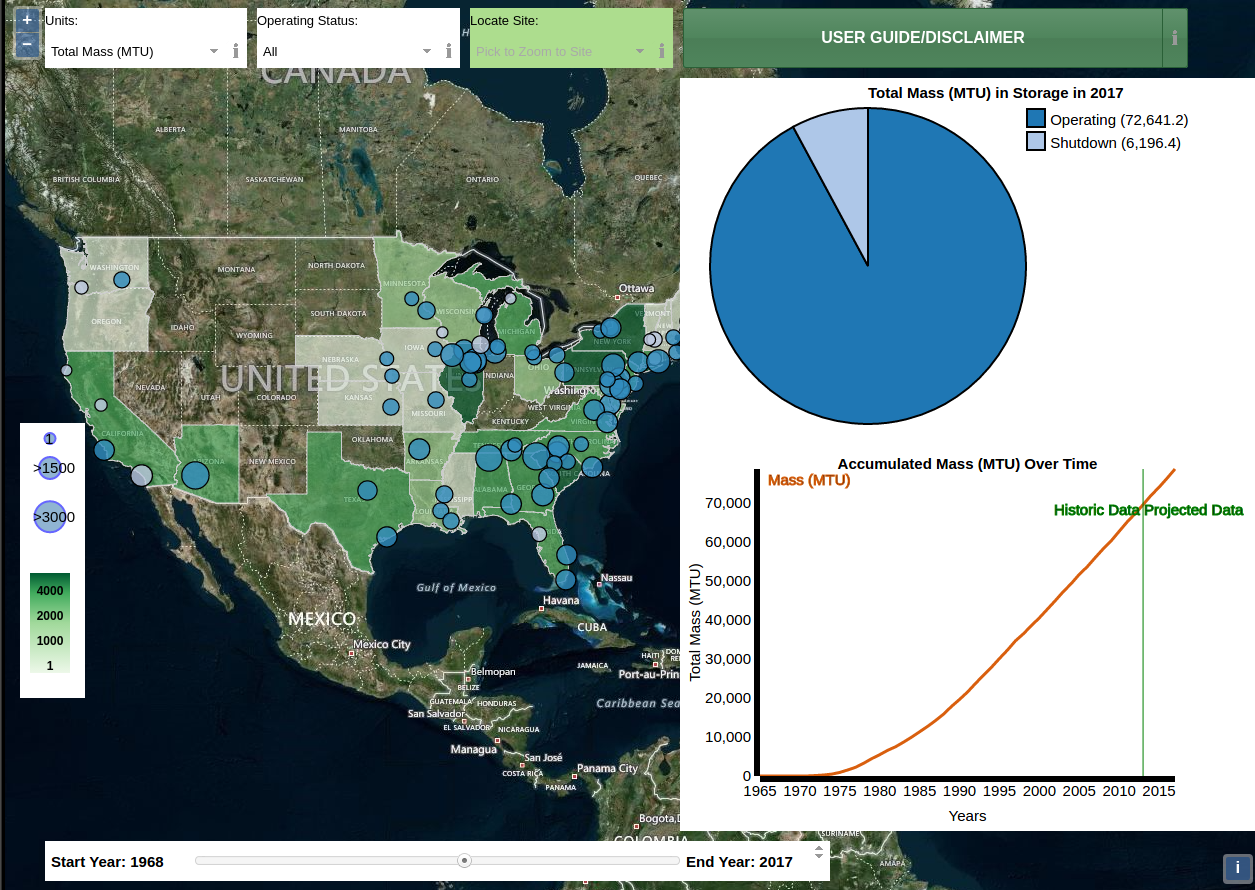
\includegraphics[height=4cm]{./images/curie_map}
		\end{center}
		\caption{ORNL CURIE map of nuclear waste. \cite{ornl_centralized_2016}.}
		\label{fig:curie_map}
	\end{figure}

\end{frame}

\begin{frame}
	\frametitle{MTHM*km For Different Reactors}
	\begin{table}[h]
		\centering
		\caption {Reactors with relatively small spent fuel transportation burden $ [MTHM\cdot km]$.}
		\scalebox{0.86}{
			\begin{tabular}{|c|c|c|c|}
			\hline
			Reactor & State & $MTHM*km$ & License Area [$km^2$]  \\ \hline
			Clinton & Illinois &  \textbf{77,352,339} & \textbf{57.87}   \\ \hline
			Dresden & Illinois &  \textbf{77,663,969} & 3.856   \\ \hline
			Peach Bottom & Pennsylvania & 85,563,135 & 2.509   \\ \hline
			Indian Point &   New York & 84,097,374 & .967   \\ \hline
			Yucca Mountain & Nevada & 209,575,157 & N/A \\ \hline
				
	\end{tabular}}
	\end {table}
			
			
	\begin{table}[h]
			\centering
			\caption {Transportation Burden for Each Case}
			%\scalebox{0.60}{
			\begin{tabular}{|c|c|c|}
				\hline
				Case & Transportation Burden [$MTHM\cdot km$] & NV\\
				\hline
				Yucca & 209,575,157  & 0\\
				Clinton & 77,352,339 & 1 \\
				\hline
			\end{tabular}
			%}
	\end{table}
\end{frame}
%%%%%%%%%%%%%%%%%%%%%%%%%%%%%%%%%
%%%%%%%%%%%%%%%%%%%%%%%%%%%%%%%%%
\subsection{Site Appropriateness}

\begin{frame}
	\frametitle{Site Appropriateness}
	\begin{figure}[!h] 
		\centering
		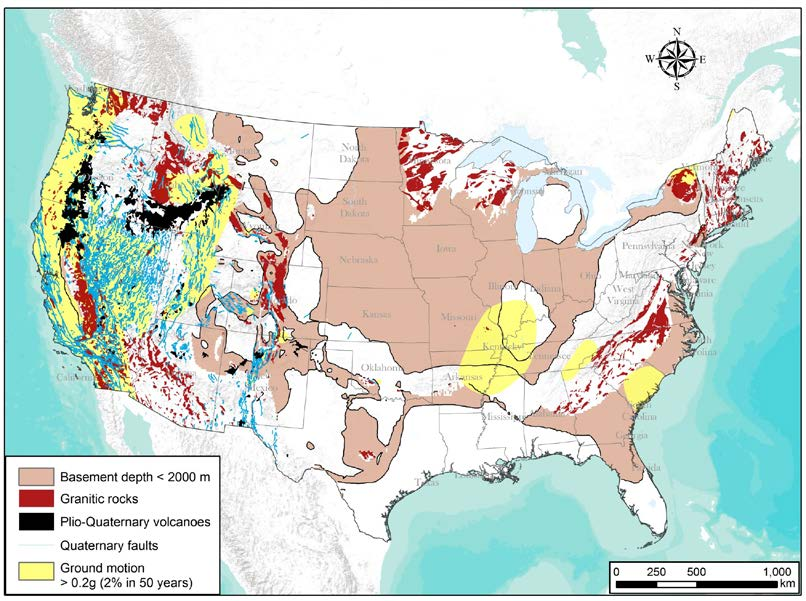
\includegraphics[width=0.6\columnwidth]{./images/cbrock.png}	
		\caption{From \cite{perry_gis_2015}, a map of areas in the US with 
				crystalline basement rock at less than 2000 meters depth. Pink
				areas suitable for borehole repositories.}
		\label{fig:cbrock}
	\end{figure}
	
\end{frame}

\begin{frame}
	\frametitle{Site Appropriateness}
	\begin{columns}
		\begin{column}{.49\columnwidth}
			\begin{figure}[h]
				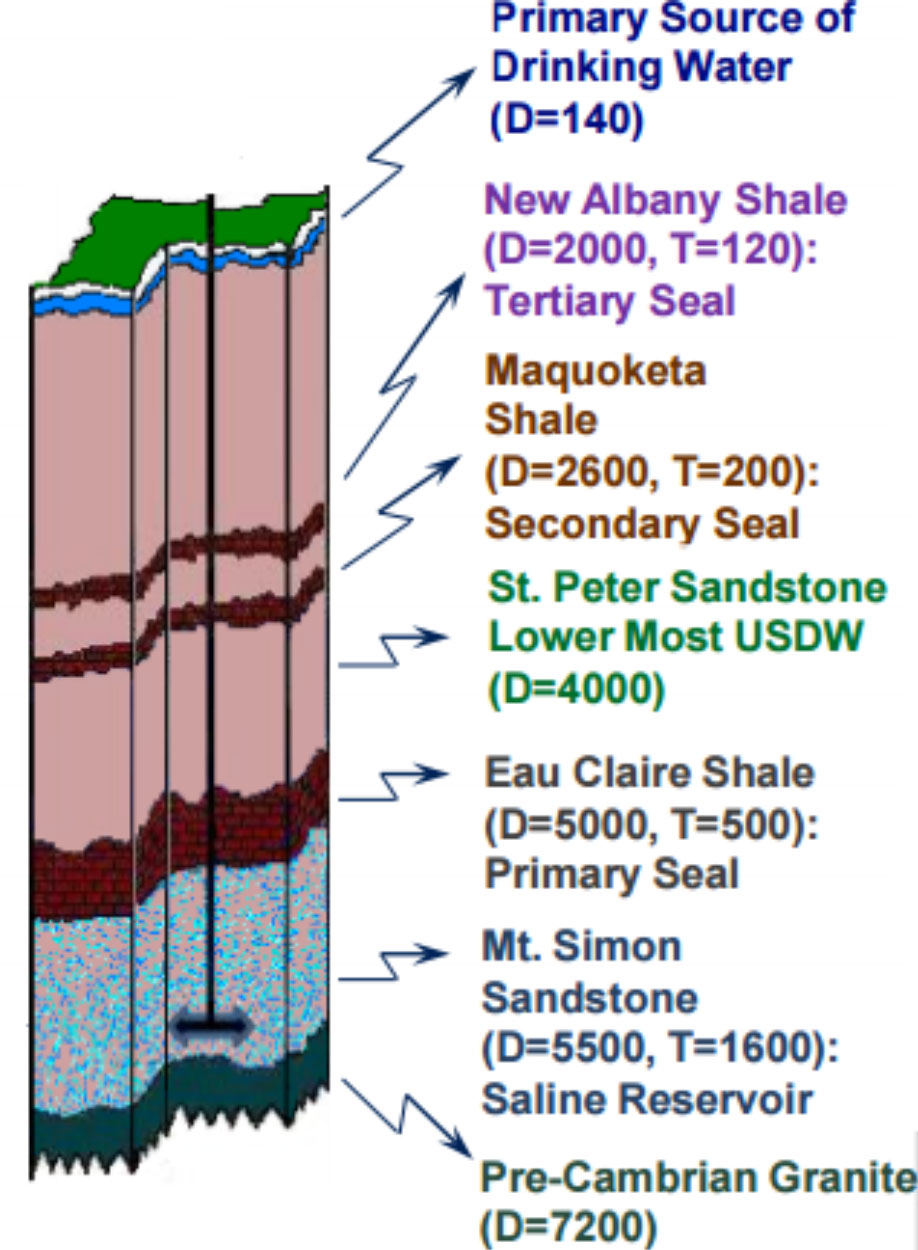
\includegraphics[width=0.75\columnwidth]{./images/Stratigraphy-Decatur.jpg}	
				\caption{Stratigraphy of the Decatur Region, D is depth in feet. \cite{mcdonald_illinois_2012}.}
				\label{fig:Stratigraphy}
			\end{figure}
		\end{column}
	\begin{column}{.49\columnwidth}
	\begin{table}[h]
		\caption {Site Appropriateness for Each Case}
		\begin{tabular}{|c|c|}
			\hline
			Case & Site Appropriateness \\
			\hline
			Yucca & 1 \\
			Clinton & 1 \\
			\hline
		\end{tabular}
	\end{table}
	\end{column}
	\end{columns}
\end{frame}


%%%%%%%%%%%%%%%%%%%%%%%%%%%%%%%%%
%%%%%%%%%%%%%%%%%%%%%%%%%%%%%%%%%
\subsection{Workforce Utilization}

\begin{frame}
	\frametitle{Workforce Utilization}
	\begin{itemize}
		\item Local Talent (nuclear experts)
		\item Transport, Catering and Lodging services
		\item 700 employees for Clinton \cite{exelon_clinton_2016}
		\item Yucca Mountain = $2,000$ - $5,000$ jobs \cite{riddel_economic_2003}
		\item The experts are no longer in Yucca after defunding of project.
	\end{itemize}
	
	\begin{table}[h]
		\centering
		\caption {Workforce Utilization for Each Case}
		%\scalebox{0.60}{
		\begin{tabular}{|c|c|}
			\hline
			Case & Workforce Utilization \\
			\hline
			Yucca & 0 \\
			Clinton & 1 \\
			\hline
		\end{tabular}
		%}
	\end{table}
\end{frame}


%%%%%%%%%%%%%%%%%%%%%%%%%%%%%%%%%
%%%%%%%%%%%%%%%%%%%%%%%%%%%%%%%%%
\subsection{Consent Basis}		

\begin{frame}
	\frametitle{Consent Basis}
	\begin{itemize}
		\item Consent-Basis approach to siting is crucial \cite{ayers_blue_2012,doe_designing_2016,jenkins-smith_public_2013,freeze_siting_2015}
		\item Communities near nuclear facilities are more likely to volunteer \cite{olsson_experiences_2013}
		\item Clinton Pays \$15 million in property taxes \cite{brady-lunny_dewitt_2016}
		\item Yucca was known as "Screw Nevada Bill" - strong opposition
	\end{itemize}
\end{frame}
		
\begin{frame}
	\frametitle{Consent Basis Metric: NMWPC}
	Nuclear MW Per Capita (NMWPC)
	\begin{table}[h]
		\centering
		\caption {NMWPC values for different states}
		\scalebox{0.60}{
			\begin{tabular}{|c|c|c|c|c|}
				\hline
				State & Net Nuclear Capacity (MW) & Census Population & NMWPC ($10^{-3}$) \\ \hline
				South Carolina & 6,486 & 4,625,401 & 1.4  \\ \hline
				Alabama & 5,043 & 4,780,127 & 1.05 \\ \hline
				Vermont & 620 & 625,745 & .99 \\ \hline
				Illinois & 11,441 & 12,831,549 & .89 \\ \hline
				Nevada & 0 & 2,705,000 & 0 \\ \hline
				Average Nuclear States & 101,167 & 265,386,569 & .38 \\ \hline
				Average National & 101,167 & 309,300,000 & .33 \\ \hline
			\end{tabular}
		}
	\end{table}
	
	\begin{table}[h]
		\centering
		\caption {NMWPC values for Each Case}
		\begin{tabular}{|c|c|c|}
			\hline
			Case & NMWPC & NV \\
			\hline
			Yucca & 0 & 0\\
			Clinton & .89 & .635\\
			\hline
		\end{tabular}
	\end{table}
\end{frame}


%%%%%%%%%%%%%%%%%%%%%%%%%%%%%%%%%
%%%%%%%%%%%%%%%%%%%%%%%%%%%%%%%%%
\subsection{Site Access}

\begin{frame}
	\frametitle{Site Access}
	\begin{itemize}
		\item Railway Access
		\item Proximity to other power plants
		\item Illinois Division of Nuclear Safety
		\item Traversal of Land:\\Yucca : 955 counties, 177 million people \cite{halstead_yucca_2011}
	\end{itemize}
	\begin{figure}[!h] 
		\centering
		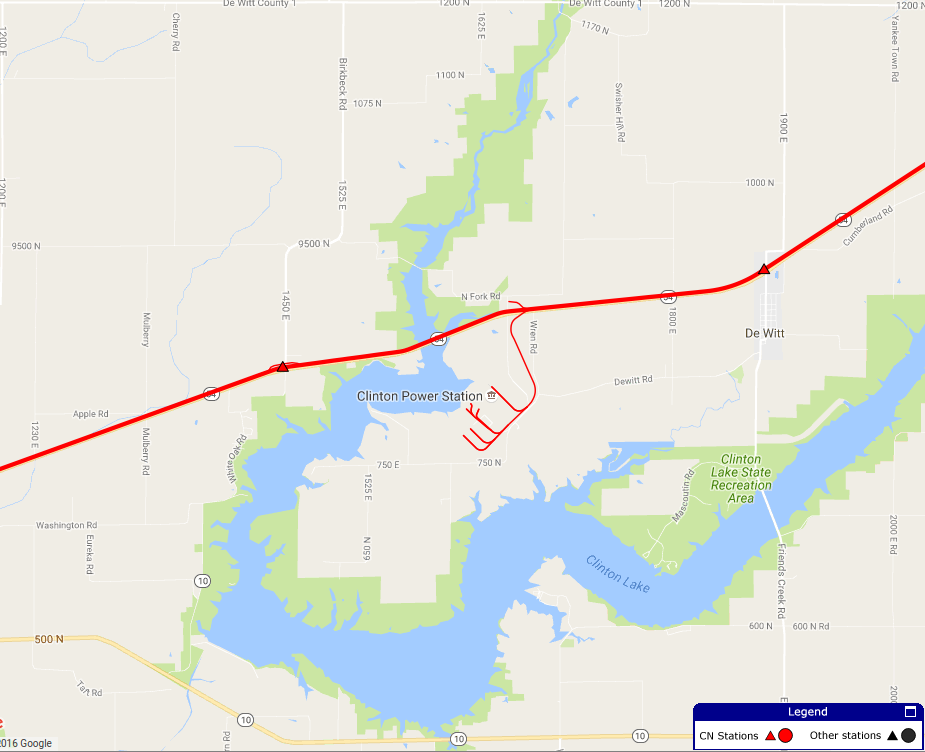
\includegraphics[width=0.4\columnwidth]{./images/cnmap.png}	
		\caption{From \cite{canadian_national_railway_company_canadian_2016}, a map of Clinton Power Station in Clinton,IL
			with the Canadian National rail passing through.}
		\label{fig:cnmap}
	\end{figure}
\end{frame}

\begin{frame}
	\frametitle{Site Access}
	
	\begin{figure}[htbp!]
		\begin{center}
			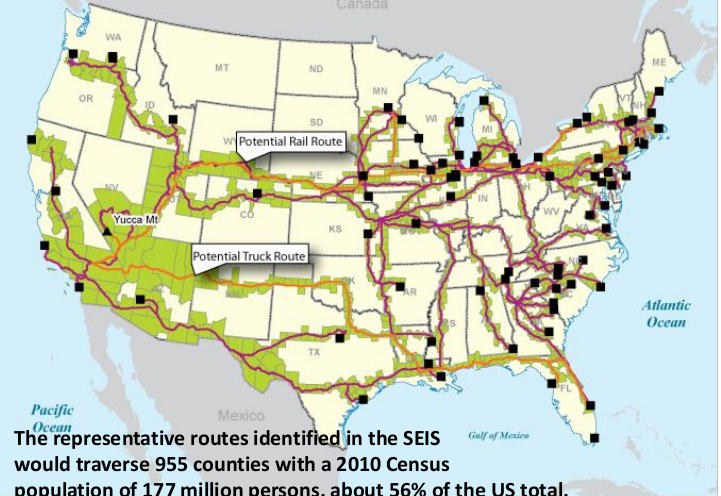
\includegraphics[height=3.5cm]{./images/yucca_route.png}
		\end{center}
		\caption{Yucca Mountain Project Estimated Route \cite{halstead_yucca_2011}.}
		\label{fig:yucca_route}
	\end{figure}
	\begin{table}[h]
		\centering
		\caption {Site Access for Each Case}
		\scalebox{0.80}{
		\begin{tabular}{|c|c|}
			\hline
			Case & Site Access \\
			\hline
			Yucca & 0 \\
			Clinton & 1 \\
			\hline
		\end{tabular}}
	\end{table}
\end{frame}



%%%%%%%%%%%%%%%%%%%%%%%%%%%%%%%%%
%%%%%%%%%%%%%%%%%%%%%%%%%%%%%%%%%
\subsection{Expediency}

\begin{frame}
	\frametitle{Expediency}
	\begin{itemize}
		\item Existing Infrastructure \\ Fuel Handling Facility \\ Railway
		\item Quicker Acceptance of SNF = less dry casks built
		\item 5 years arbitrarily chosen for time of fuel handling facility
	\end{itemize}
	\begin{table}[h]
		\centering
		\caption {Expediency in Each Case}
		\begin{tabular}{|c|c|c|}
			\hline
			Case & Time Saved [y] & NV \\
			\hline
			Yucca & 0 & 0\\
			Clinton & 5 & 1 \\
			\hline
		\end{tabular}
	\end{table}
\end{frame}